\documentclass[12pt, a4paper]{article}
\usepackage[T1]{fontenc}
\usepackage{graphicx}
\usepackage{mathptmx}
\usepackage{listings}
\usepackage{xcolor}
\usepackage{ragged2e}
\date{}
\pagenumbering{gobble}

\graphicspath{{./img}}

\definecolor{mGreen}{rgb}{0,0.6,0}
\definecolor{mGray}{rgb}{0.5,0.5,0.5}
\definecolor{mPurple}{rgb}{0.58,0,0.82}
\definecolor{backgroundColour}{rgb}{0.95,0.95,0.92}

\lstset{
  language=C,                % choose the language of the code
  numbers=left,                   % where to put the line-numbers
  stepnumber=1,                   % the step between two line-numbers.
  numbersep=5pt,                  % how far the line-numbers are from the code
  backgroundcolor=\color{white},  % choose the background color. You must add \usepackage{color}
  showspaces=false,               % show spaces adding particular underscores
  showstringspaces=false,         % underline spaces within strings
  showtabs=false,                 % show tabs within strings adding particular underscores
  tabsize=2,                      % sets default tabsize to 2 spaces
  captionpos=b,                   % sets the caption-position to bottom
  breaklines=true,                % sets automatic line breaking
  breakatwhitespace=true,         % sets if automatic breaks should only happen at whitespace
  title=\lstname,                 % show the filename of files included with \lstinputlisting;
}


\begin{document}

  \begin{flushleft}
    NAMA           : RADINAL SHIDIQ SARAGIH

    NPM            : 5520123104

    KELAS/ANGKATAN : IF-C 2023

    MATA KULIAH    : STRUKTUR DATA
  \end{flushleft}

  \begin{center}
    \section*{DESKRIPSI PROGRAM SINGLE LINKED LIST NON-CONTIGUOUS}
  \end{center}

  \vspace{0.5cm}

  Struktur data Linked List adalah struktur data yang dapat dibuat oleh seorang
  programmer untuk menyimpan data secara dinamis. Linked List pada dasarnya dapat
  digambarkan sebagai sekumpulan data yang dihubungkan satu sama lain di memori.

  Struktur data Single Linked List terdapat beberapa jenis dan masing-masing memiliki
  kelebihan dan kekurangan masing-masing. Yang akan dideskripsikan disini adalah
  Linked List yang Single, artinya hanya menyimpan satu penunjuk ke data selanjutnya,
  dan Non-Contiguous yang artinya di data terakhir tidak menunjuk ke data pertama.

  Struktur data Linked List sangat penting untuk dipahami karena selain memberikan
  kemampuan untuk seorang programmer agar dapat membuat sebuah struktur data sesuai
  kebutuhannya hingga dapat membuat program lebih efisien, Linked List tersendiri
  adalah konsep dasar dari banyak struktur data lain yang lebih kompleks seperti
  tree dan graph.

  Linked List dapat dibuat diberbagai bahasa pemograman, dan yang paling umum digunakan
  adalah C, karena C tidak memberikan struktur data lain di dalam library standarnya.

  Perbedaan implementasi diantara bahasa pemograman bergantung kepada sebagaimana
  bahasa tersebut memeberikan cara seorang programmer untuk membuat tipe datanya
  sendiri.

  Dan bedasarkan tugas, dicantumkan program linked list didalam bahasa C++, yaitu sebagai berikut.

  \vspace{0.5cm}
  \lstinputlisting{source_file/linkedlist.cpp}
  \vspace{0.5cm}

  \newpage

  Program ini akan meng-output sebuah menu, yang akan memberikan beberapa pilihan
  untuk menambah, menghapus, menghapus tengah, dan juga memperlihatkan data di sebuah
  linked list.

  Dan jika user meng-input sebuah angka, angka tersebut akan diproses dan
  digunakan untuk menentukan fungsi apa dalam program yang akan dipanggil untuk
  memanipulasi linked list.

  Output dari program ini adalah sebagi berikut.

  \begin{center}
    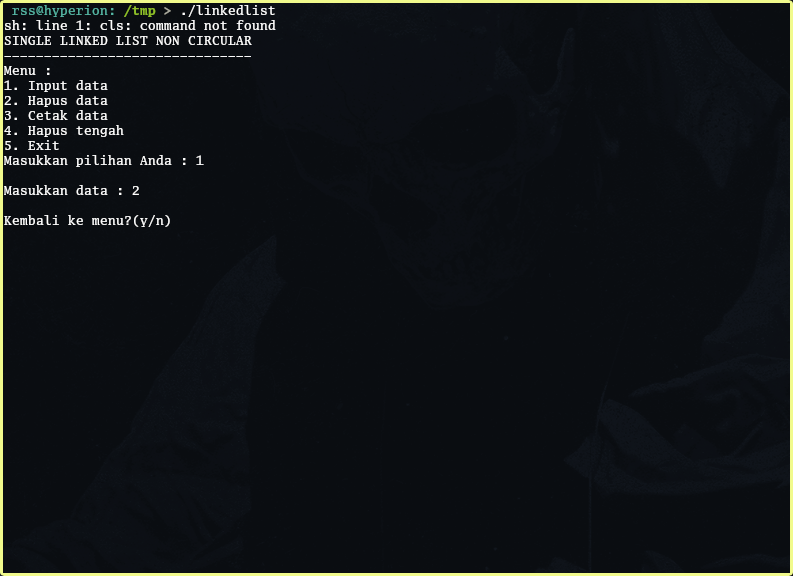
\includegraphics[scale=0.3]{ORGSLLNCINPUT}
  \end{center}

  Di menu program juga terdapat pilihan untuk meng-print atau meng-outputkan
  data dengan representasi Linked List.

  \begin{center}
    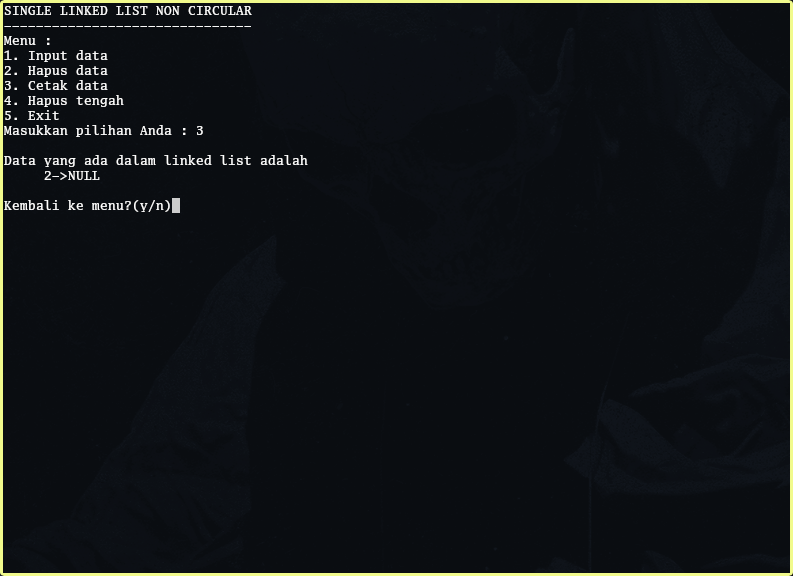
\includegraphics[scale=0.3]{ORGSLLNCOUTPUT}
  \end{center}

  Bedasarkan perintah tugas yang telah diberikan yaitu.

  \begin{center}
  ``Silahkan kalian coba deskripsi program dibawah ini, jika terjadi error sintak, selsaikan logikanya dan apa keluaran dari list program tersebut``
  \end{center}

  Dari program tersebut dapat dibuat beberapa penyesuaian dan perbaikan dalam hal
  kerapihan dan juga kompabilitas program dengan sistem operasi lain.

  Di dalam source code tersebut dapat dirubah beberapa hal, antara lain.

  \begin{itemize}
    \item Mengurangi pemakaian variabel global agar lebih mudah dibaca.
    \item Merubah penamaan variabel dan fungsi agar lebih mudah dipahami.
    \item Mengurangi pemakaian library yang tidah digunakan.
    \item Memberikan logika tambahan untuk membersihkan terminal/konsol agar
      dapat memanggil perintah yang sesuai di sistem operasi selain windows.
    \item Optimisasi algoritma yang kurang optimal dan penanganan input yang lebih aman.
    \item Menyerdehanakan beberapa operasi kedalam fungsi tersendir.
    \item Menyesuaikan banyak bentuk program yang memanfaatkan fungsionalitas
      bahasa C kedalam bentuk yang lebih C++.
    \item Menambah fungsi tambahan yang dipanggil ketika program selesai untuk
      membersihkan memori yang telah dialokasikan, tidak harus dilakukan untuk
      kasus program ini namun merupakan best-practice untuk selalu membersihkan
      semua memori yang telah secara manual dialokasikan ke heap.
  \end{itemize}

  Maka setelah melakukan penyesuaian didapatkan sebagi berikut.

  \vspace{0.5cm}
  \lstinputlisting{source_file/SingleLinkedListNC.cpp}
  \vspace{0.5cm}

  Dan dari output program tersebut didapatkan sebagai berikut.

  \begin{center}
    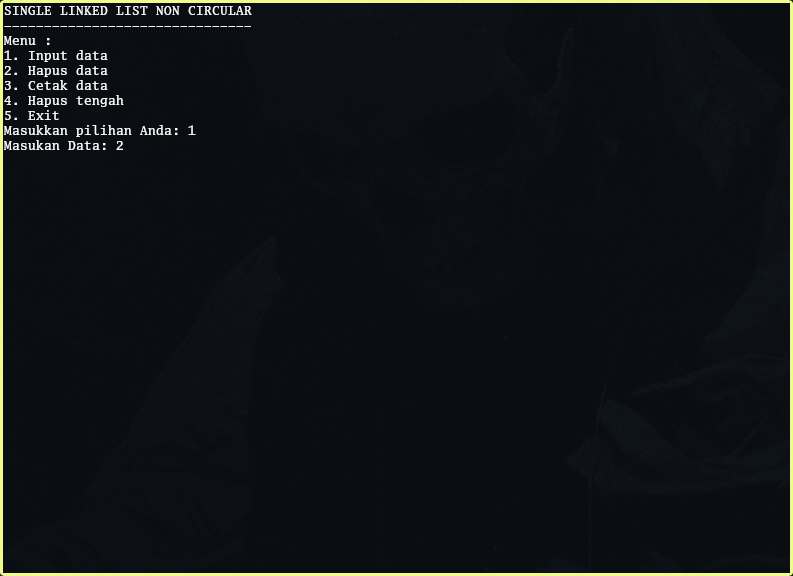
\includegraphics[scale=0.4]{REVSLLNCINPUT}
  \end{center}

  Dan juga sama seperti sebelumnya, di menu program juga terdapat pilihan
  untuk meng-print atau meng-outputkan data dengan representasi Linked List.

  \begin{center}
    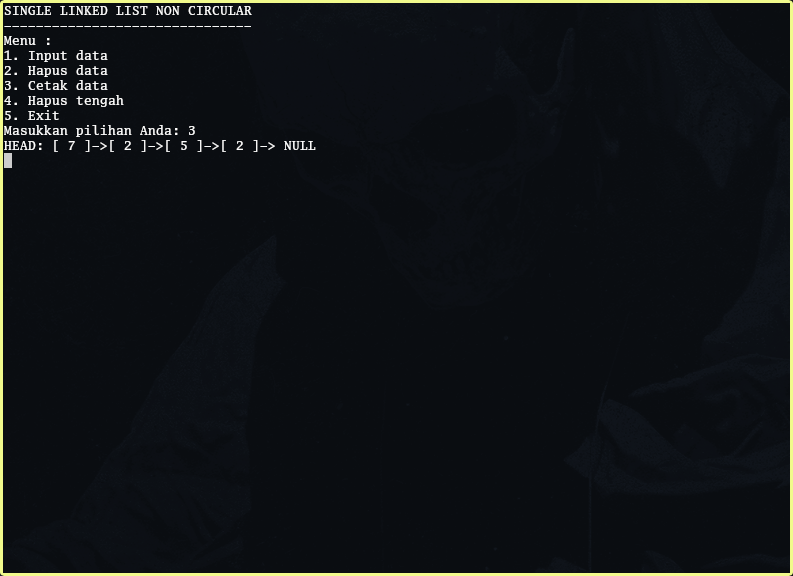
\includegraphics[scale=0.4]{REVSLLNCOUTPUT}
  \end{center}

  Namun terdapat beberapa perbedaan logika dengan program aslinya dengan revisi
  yang ini, salah satunya pada operasi menghapus tengah.

  Di program pertama terdapat fungsi hapus tengah sebagai berikut.

  \vspace{0.5cm}
  \begin{lstlisting}
    void hapus_tengah()
    {
      float posisi_tengah;

      //'jumlah' dibagi 2, kemudian dibulatkan ke bawah
      posisi_tengah = float(hitung_node()/2);

      int simpan, simpan2;

      if(head==NULL) {
        cout<<"\nlinked list kosong, penghapusan tidak bisa dilakukan"<<endl;
      } else
    {
        if(hitung_node()<=2){
          hapus();
        } else if(hitung_node()==3){
          curr2 = head;
          simpan_pos1 = curr2->next;
          //menyambungkan node awal dengan node akhir
          curr2->next = curr2->next->next;
          simpan2 = simpan_pos1->data;
          cout<<"\ndata yang dihapus adalah "<<simpan2<<endl;

          simpan_pos1->next = NULL;
          delete simpan_pos1;
        } else if(hitung_node()>3) {
          curr3 = head;
          //menempatkan pointer di posisi "sebelum" tengah
          for(float i = 0; i<posisi_tengah-1; i++){
            curr3 = curr3->next;
            simpan_pos2 = curr3;
          }
          curr4 = head;
          //menempatkan pointer di posisi tengah
          for(float i = 0; i<posisi_tengah; i++){
            curr4 = curr4->next;
            simpan_pos3 = curr4;
          }
          simpan = simpan_pos3->data;
          cout<<"\ndata yang dihapus adalah "<<simpan<<endl;
          //menyambungkan node sebelum 'node tengah' dengan node sesudah 'node tengah'
          simpan_pos2->next = simpan_pos3->next;
          //hapus node
          simpan_pos3->next = NULL; //memutus hubungan node sebelum dihapus
          del = simpan_pos3;
          delete del;
        }
      }
    }
  \end{lstlisting}
  \vspace{0.5cm}

  Fungsi ini menggunakan banyak for-loop untuk menemukan pointer data sebelum
  tengah dan sesudah tengah, maka ada proses pencarian linier yang dilakukan
  beberapa kali hingga dapat memperlambat proses penghapusan tengah jika linked
  list memiliki banyak data. Dan dalam penghapusan fungsi ini akan menghapus
  data sebelum data di tengah bukan data di tengah itu sendiri.

  Maka didalam revisi telah di optimisasi dan membuat agar menghapus nilai
  ditengah, hingga didapatkan sebagai berikut.

  \vspace{0.5cm}
  \begin{lstlisting}
    void
    hapus_node_tengah(LinkedList* linked_list)
    {
      size_t jumlah_node = hitung_node(linked_list);

      if (linked_list->kosong()) {
        std::cout << "Linked List Kosong!\n";
      } else if (jumlah_node <= 2) {
        // jika jumlah node <= 2, hapus saja dari head
        hapus_node_awal(linked_list);
      } else {

        size_t index_node_tengah = jumlah_node / 2;

        Node* node_tengah = linked_list->head;
        Node* node_sebelum_tengah = linked_list->head;

        // iterasikan sebanyak jumlah node tengah
        for (size_t i = 0; i < index_node_tengah; i++) {

          // simpan node sebelum node tengah
          node_sebelum_tengah = node_tengah;

          // simpan node tengah
          node_tengah = node_tengah->next;
        }

        // putuskan hubungan node tengah dengan node selanjutnya
        node_sebelum_tengah->next = node_tengah->next;

        // dapatkan data yg disimpan
        size_t data_node_tengah = node_tengah->data;

        // hapus data di tengah
        delete node_tengah;

        // print data node yang dihapus
        std::cout << "Data Dihapus: " << data_node_tengah << "\n";
      }
    }
  \end{lstlisting}
  \vspace{0.5cm}

  Perbedaan paling signifikan adalah didalam fungsi ini adalah berkurangnnya
  jumlah for-loop yang digunakan. Secara logika ini dimungkinkan karena
  for-lop tersebut akan mencari dari node pertama hingga (jumlah\_node / 2) - 1.

  Dan di tiap iterasi akan disimpan dua buah pointer node, yaitu node\_tengah
  dan node\_sebelum\_tengah.

  node\_tengah akan menunjuk ke node yang ditengah, di tiap iterasikan di for-loop
  nilai variabel ini akan menunjuk ke data selanjutnya hingga ketika for-loop
  selesai akan memberikan pointer yang sesuai.

  node\_sebelum\_tengah tengah menyimpan nilai ponter yang ditunjuk node\_tengah
  sebelum ia dirubah menjadi node selanjutnya, maka ketika for-loop selesai akan
  menunjuk nilai terakhir node\_tengah sebelumnya.

  maka dengan itu pencarian akan dilakukan satu kali dan iterasi akan hanya berjumlah
  sampai index tengah.

  Selain perbedaan tersebut juga terdapat dalam fungsi-fungsi lain yang telah
  disesuaikan agar memanfaatkan variabel local dibandingkan variabel global, karena
  membuat alur program sulit untuk diikuti dan dibaca.

  Terdapat juga perbedaan dalam cara membersihkan layar konsol atau terminal. Di dalam
  program sebelumnya terdapat pemanggilan fungsi system(), yang akan memanggil perintah
  terminal/shell bernama "cls" yang akan membersihkan layar konsole di windows.

  Maka karena saya sendiri menggunakan Linux pemanggilan system("cls") tidak akan
  menghasilkan respon yang sama di terminal linux atau pun mac-os
  (linux dan mac-os memiliki shell yang serupa) maka dengan menggunakan logika pre-processor.
  dibuat sebagai berikut.

  \vspace{0.5cm}
  \begin{lstlisting}
    void
    bersihkan_layar()
    {
    #ifdef _WIN32
      system("cls");
    #endif // untuk windows

    #ifdef __linux__
      system("clear");
    #endif // untuk linux
    }
  \end{lstlisting}
  \vspace{0.5cm}

  Disini dengan menggunakan \#ifdef, yang akan mengecek jika sebuah label telah
  didefinisikan atau ada, dapat dilakukan pengaturan bagaimana pemanggilan
  sistem dilakukan diantara sistem operasi yang berbeda.

  Kedua label \_WIN32 dan \_\_linux\_\_ dalah label yang akan didefiniskan
  oleh kompiler diwaktu proses kompilasi.

  Jadi, secara fungsionalitas tidak terjadi banyak perubahan, namun revisi yang
  saya buat memberikan beberapa perbaikan dan perkembangan terhadap source code
  agar lebih mudah dipahami dan memiliki Kompabilitas antar OS yang lebih baik.

  Untuk mendeskripsi kan bagaimana operasi terhadap linked list dilakukan, kita bisa
  mulai dari fungsi tambah\_node() yang akan menambah node baru di awal list.

  \vspace{0.5cm}
  \begin{lstlisting}
    void
    tambah_node(LinkedList* linked_list, int data)
    {
      Node* node_baru = new Node;
      node_baru->data = data;

      // jika list kosong tambah di head
      if (linked_list->kosong()) {
        linked_list->head = node_baru;
        linked_list->tail = linked_list->head;
      } else {
        // tambah di tail
        linked_list->tail->next = node_baru;
        linked_list->tail = node_baru;
      }
    }
  \end{lstlisting}
  \vspace{0.5cm}

  Penambahan node di awal di fungsi dapat dijabarkan sebagai langkah-langkah
  sebagai berikut.

  \begin{enumerate}

    \item Alokasikan Memory untuk node baru.
    \item Cek jika list masih kosong.
    \item jika kosong simpan node baru di Head.
    \item jika tidak kosong tambah di Tail.
  \end{enumerate}

  Lalu juga ada hapus\_node\_awal(). Fungsi ini akan menghapus node diawal list.

  \vspace{0.5cm}
  \begin{lstlisting}
    void
    hapus_node_awal(LinkedList* linked_list)
    {
      if (linked_list->kosong())
        return;

      Node* node_dihapus = linked_list->head;
      int data_dihapus = node_dihapus->data;

      // cek jika tidak ada node setelah head
      if (linked_list->head->next != NULL) {
        // jika ada set head ke node berikutnya
        linked_list->head = linked_list->head->next;
      } else {
        // jika tidak ada head == NULL
        linked_list->head = NULL;
      }

      delete node_dihapus;

      std::cout << "Data Dihapus: " << data_dihapus << "\n";
    }
  \end{lstlisting}
  \vspace{0.5cm}

  Penghapusan node di awal di fungsi dapat dijabarkan sebagai langkah-langkah
  sebagai berikut.

  \begin{enumerate}
    \item Cek jika list kosong, jika kosong jangan lakukan apapun.
    \item Simpan pointer ke node yang ditunjuk Head.
    \item Cek jika ada node setelah head.
    \item jika ada node setelah head, buat head menunjuk ke node berikutnya.
    \item jika idak ada node setelah head, artinya list kosong, maka buat Head menunjuk ke NULL.
    \item De-alokasikan/hapus node yang disimpan tadi.
  \end{enumerate}

  Juga ada fungsi yang akan menampilkan data yang tersimpan yaitu print\_linked\_list().

  \vspace{0.5cm}
  \begin{lstlisting}
    void
    print_linked_list(LinkedList* linked_list)
    {

      if (linked_list->kosong()) {
        std::cout << "Linked List Kosong!\n";
      } else {

        Node* node = linked_list->head;

        std::cout << "HEAD: ";

        // iterasikan seluruh node dan
        // print nilai mereka
        while (node != NULL) {
          std::cout << "[ " << node->data << " ]->";
          node = node->next;
        }

        std::cout << " NULL\n";
      }
    }
  \end{lstlisting}
  \vspace{0.5cm}

  Fungsi ini cukup sederhana namun dijabarkan sebagai langkah-langkah
  sebagai berikut.

  \begin{enumerate}
    \item Cek jika list kosong, jika kosong berikan respon bahwa list kosong.
    \item Jika list tidak kosong, iterasikan linked list menggunakan variable
      pointer yang akan membantu iterasi, lakukan iterasi hingga variable tersebut bernilai NULL.
    \item Di tiap iterasi print nilai node dan kemudian rubah variable
      node tadi untuk menunjuk ke node selanjutnya.
  \end{enumerate}

  Terdapat juga fungsi yang membantu fungsi hapus\_tengah() untuk mencari
  jumlah node yang terdapat dalam list, yaitu hitung\_node().

  \vspace{0.5cm}
  \begin{lstlisting}
    size_t
    hitung_node(LinkedList* linked_list)
    {
      size_t jumlah_node = 0;

      // jika kosong jumlah == 0
      if (linked_list->kosong())
        return jumlah_node;

      Node* node = linked_list->head;

      // iterasikan seluruh node di list
      // hitung satu persatu
      while (node != NULL) {
        ++jumlah_node;
        node = node->next;
      }

      return jumlah_node;
    }
  \end{lstlisting}
  \vspace{0.5cm}

  Fungsi ini juga cukup sederhana namun jika dijabarkan sebagai langkah-langkah
  maka didapatkan.

  \begin{enumerate}
    \item Buat variable yang akan menyimpan jumlah node, set ke 0.
    \item Cek jika list kosong, jika kosong return nilai variable
      jumlah node tadi yang bernilai 0.
    \item Jika list tidak kosong, iterasikan seluruh list dari head, dan increment nilai
      variable jumlah node tadi dengan 1, lakukan hingga node yang menunjuk ke head tadi
      bernilai NULL.
    \item Return nilai variable jumlah node;
  \end{enumerate}

  Dan terakhir, yaitu hapus\_node\_tengah(), seperti telah dijelaskan sebelumnya
  fungsi ini akan menghapus node di tengah linked list.

  \vspace{0.5cm}
  \begin{lstlisting}
    void
    hapus_node_tengah(LinkedList* linked_list)
    {
      size_t jumlah_node = hitung_node(linked_list);

      if (linked_list->kosong()) {
        std::cout << "Linked List Kosong!\n";
      } else if (jumlah_node <= 2) {
        // jika jumlah node <= 2, hapus saja dari head
        hapus_node_awal(linked_list);
      } else {

        size_t index_node_tengah = jumlah_node / 2;

        Node* node_tengah = linked_list->head;
        Node* node_sebelum_tengah = linked_list->head;

        // iterasikan sebanyak jumlah node tengah
        for (size_t i = 0; i < index_node_tengah; i++) {

          // simpan node sebelum node tengah
          node_sebelum_tengah = node_tengah;

          // simpan node tengah
          node_tengah = node_tengah->next;
        }

        // putuskan hubungan node tengah dengan node selanjutnya
        node_sebelum_tengah->next = node_tengah->next;

        // dapatkan data yg disimpan
        size_t data_node_tengah = node_tengah->data;

        // hapus data di tengah
        delete node_tengah;

        // print data node yang dihapus
        std::cout << "Data Dihapus: " << data_node_tengah << "\n";
      }
    }
  \end{lstlisting}
  \vspace{0.5cm}

  Fungsi ini terlihat kompleks namun jika dijabarkan cukup sederhana.

  \begin{enumerate}
    \item simpan jumlah node yang diberikan fungsi hitung\_node() ke
      sebuah variable.
    \item cek jika list kosong, jika kosong berikan respon bahwa list kosong.
    \item cek jika list tidak kosong, dan memiliki jumlah node <= 2, hapus saja
      node menggunakan hapus\_node\_awal().
    \item Jika list tidak kosong dan juga tidak memiliki jumlah node <= 2, lakukan
      proses penghapusan tengah.
      \begin{itemize}
        \item Dapatkan nilai index tengah dengan membagi jumlah\_node dengan 2, simpan di variable index node tengah.
        \item Buat dua variable pointer ke Node, variable untuk sebelum node tengah, dan variable untuk node tengah.
        \item iterasikan sebanyak jumlah index node tengah tadi, dan di tiap iterasi buat variable yang menyimpan
          node sebelum tengah untuk menyimpan nilai node tengah yang disimpan di variable node tengah, lalu buat
          node tengah tersebut untuk menunjuk ke node selanjutnya.
        \item selesai iterasi, mulai proses penghapusan. Buat pointer yang dimiliki node sebelum tengah untuk menunjuk
          ke node setelah node tengah.
        \item Dan terakhir de-alokasi/hapus node tengah tersebut.
      \end{itemize}
  \end{enumerate}

  Dan untuk fungsi-fungsi lain didalam program tidak perlu dijabarkan karena sangat sederhana dan dapat dijabarkan
  dengan mudah.

  \begin{center}
    ......
  \end{center}

\end{document}
